\part{Prérequis}

\textbf{Problème d'optimisation dans $\mathbb{R}$} Il s'agit de trouver une valeur pour laquelle une fonction  est minimale.

\begin{figure}[H]
    \centering
    \tikzsetnextfilename{produit_cartesien}
    \begin{tikzpicture}
        \draw[->] (0,-.5) -- (0,5);
        \draw[->] (-.5,0) -- (2,0) node[below] {$a$} node{$\times$} -- (6,0) node[below] {$b$} node{$\times$} -- (10,0);
        \draw [domain=1.25:8.75, samples=80, smooth] plot (\x, {(\x - 3.5)^2/10 + 1.25}) node[right] {$\phi(x)\in \mathcal{C}^0$};
        \draw[dashed] (0,1.25) node[left] {$\phi(x^\star) = \min_{x\in I}\phi(x)$} -- (3.5,1.25) -- (3.5,0) node[below] {$x^\star$};
    \end{tikzpicture}
    %\caption{Caption}
    %\label{fig:my_label}
\end{figure}

\begin{theo}[Théorème des valeurs extrêmes] \label{theo:valextr}
    Soit $\phi$ une fonction définie sur un intervalle $I = \left[ a,b \right]$ de réels et à valeurs réelles. Si $\phi$ est continue, alors la fonction $\phi$ est bornée et atteint ses bornes, autrement dit, il existe deux réels $c$ et $d$ de l'intervalle $I$ tels que pour tout $x \in I$, les inégalités suivantes soient vérifiées : \[\phi(c) \leq \phi(x) \leq \phi(d)\]
\end{theo}

\begin{remark}
    Ce théorème n'est valable qu'en dimension finie
\end{remark}

\section{Les ensembles}

\begin{definition}
    Un \textbf{ensemble} est une \textit{collection} ou un groupement d'objets distincts, appelés \textit{éléments} de cet ensemble. On parle d'ensemble fini si l'on peut compter le nombre d'éléments qui s'y trouvent ($E = \left\{ 1,2,3,4 \right\}$), d'ensemble infini dénombrable si l'on peut savoir exactement tous les nombres qui s'y trouvent ($\mathbb{N},\mathbb{N}_0,\mathbb{Z},\mathbb{Q},...$) et d'ensemble infini indénombrable ($\mathbb{R}$).
\end{definition}

La théorie des ensembles prend en compte un certain nombres d'axiomes, définissant les opérations admissibles, afin d'éviter toute contradiction lors des manipulations :
\begin{description}
    \item[Axiome de l'ensemble vide.] Il existe un ensemble, noté $\emptyset$, qui ne contient aucun élément.
    \item[Axiome d'extensionalité.] Deux ensembles $A$ et $B$ sont égaux $A=B$ s'ils contiennent les mêmes éléments. Si un ensemble $A$ contient tous les éléments d'un ensemble $B$, alors $B$ est un sous-ensemble de $A$ ($B\subseteq A$). En particulier, on a $A\subseteq B$ et $B\subseteq A$ ssi $A=B$.
    \item[Axiome d'accouplement.] Si $A$ et $B$ sont deux ensembles, il existe alors un ensemble $\left\{ A,B \right\}$ qui contient $A$ et $B$ comme éléments. On admet que $\left\{ A,A \right\} = \left\{ A \right\}$. Par l'axiome d'extensionalité, nous avons que $\left\{ A,B \right\} = \left\{ B,A \right\}$.
    \item[Axiome d'union.] Soit un ensemble $\mathcal{F}$ donné dont les éléments sont eux-mêmes des ensembles. Il existe un ensemble $A=\bigcup\mathcal{F}$ contenant tous les éléments de tous les éléments de $\mathcal{F}$. En particulier, soit deux ensembles $A$ et $B$, il existe un ensemble $A\cup B=\bigcup\left\{ A,B \right\}$. Notez que cette définition assure la commutativité $A\cup B = B\cup A$ et l'associativité $(A\cup B) \cup C = A\cup (B\cup C)$ de l'union.
    \item[Schéma axiomatique de spécification.] Soit un ensemble $A$ donné et $\phi(x)$ une déclaration logique dépendant de $x\in A$, on peut former $B=\left\{ x\in A | \phi(x) \right\}$ de tous les éléments de $A$ observant $\phi(x)$.
    \item[Axiome de <<power set>>.] Pour un ensemble $A$ donné, il existe un ensemble, noté $\mathcal{P}(A), \mathfrak{P}(A)$ ou encore $2^A$, qui contient tous les sous-ensembles de $A$. Il est défini par \[B \in \mathcal{P}(A) \Longleftrightarrow B \subseteq A.\]
\end{description}
On définit ensuite l'ensemble des applications d'un ensemble $Y$ dans un ensemble $X$ par $X^Y$ ($\mathbb{R}^\mathbb{N}, \mathbb{R}^\mathbb{R}$). Comme $2$ peut être défini comme l'ensemble $\left\{ 0,1 \right\}$, $2^X$ peut désigner l'ensemble des fonctions de $X$ dans $\left\{ 0,1 \right\}$. \\

\begin{description}
    \item[Schéma axiomatique de la substitution.] Pour toute fonction $f$, l'image d'un ensemble $A$ est un ensemble $B=\left\{ f(x)|x\in A \right\}$.
    \item[Axiome d'infinité.] Il existe un ensemble $A$ qui contient l'ensemble vide et pour tout élément $x\in A$, on a aussi $x\cup\left\{x\right\}\in A$. Le plus petit ensemble de la sorte, $\left\{ \emptyset, \left\{ \emptyset \right\}, \left\{ \emptyset, \left\{ \emptyset \right\} \right\},... \right\}$, peut être identifié avec les entiers via $0=\emptyset, 1 = \left\{ \emptyset \right\}, 2 = \left\{ \emptyset, \left\{ \emptyset \right\} \right\}, ...$
    \item[Axiome de régularité.] tout ensemble $A$ non vide contient un élément $x$ avec $x\cap A = \emptyset$. Ceci exclut par exemple qu'un ensemble se contienne lui-même. De manière similaire, on peut avoir $A\in B$ ou $B\in A$, mais pas les deux.
    \item[Axiome de choix.] Soient $A$ un ensemble d'index et $\left\{ M_\alpha \right\}_{\alpha\in A}$ des ensembles non vides. Leur produit $\huge{\times}_{\alpha\in A}M_\alpha$ est non vide.
\end{description}

\begin{definition}
    Le \textbf{produit cartésien} de deux ensembles $X$ et $Y$, appelé \textbf{ensemble-produit}, est l'ensemble de tous les couples dont la première composante appartient à $X$ et la seconde à $Y$. On généralise facilement cette notion, valable pour deux ensembles, à celle de produit cartésien fini, qui est un ensemble de $n$-uplets dont les composantes appartiennent à $n$ ensembles. La généralisation à un produit cartésien infini nécessite, quant à elle, la notion de fonction.
\end{definition}

\begin{example}
    $\left\{ 1,2,3 \right\} \times \left\{ 1,2,3 \right\} = \left\{ 1,2,3 \right\}^2$
    \begin{figure}[H]
        \centering
        \tikzsetnextfilename{produit_cartesien}
        \begin{tikzpicture}
            \draw[<->] (1,0) -- (0,0) -- (0,1);
            \draw (-.5,.5) node[] {$\mathbb{R}^2$};

            \draw[<->] (5,0) -- (4,0) -- (4,1);
            \draw[->] (4,0) -- (3.5,-.5);
            \draw (3.5,.5) node[] {$\mathbb{R}^3$};

            \draw[<-] (8,1) -- (8,-.1);
            \draw[->] (7.9,0) -- (11.5,0);
            \draw plot[mark=*, mark size=.3mm] (8.5,0) -- plot[mark=*, mark size=.3mm] (8.5,.5);
            \draw plot[mark=*, mark size=.3mm] (9,0) -- plot[mark=*, mark size=.3mm] (9,.2);
            \draw plot[mark=*, mark size=.3mm] (9.5,0) -- plot[mark=*, mark size=.3mm] (9.5,-.3);
            \draw (10,0) node[below] {$\cdots$};
            \draw plot[mark=*, mark size=.3mm] (10.5,0) -- plot[mark=*, mark size=.3mm] (10.5,.5);
            \draw (7.5,.5) node[] {$\mathbb{R}^\mathbb{N} \ni$};
        \end{tikzpicture}
        %\caption{Caption}
        %\label{fig:my_label}
    \end{figure}
\end{example}

\section{Espaces métriques et topologiques}

\subsection{Bases}

\begin{definition}
    Un \textbf{espace métrique} est un espace $X$ auquel une distance $d$ est associée : $X\times X\rightarrow \mathbb{R}$ tel que pour les points arbitraires $x,y,z\in X$, on ait :
    \begin{enumerate}[label=(\roman*)]
        \item $d(x,y) \geq 0$ ;
        \item $d(x,y) = 0$ ssi $x = y$ (séparation) ;
        \item $d(x,y) = d(y,x)$ (symétrie) ;
        \item $d(x,z) \leq d(x,y) + d(y,z)$ (inégalité triangulaire).
    \end{enumerate}
    Conséquence : $|d(x,y)-d(z,y)| \leq d(x,z)$
\end{definition}

\begin{example}
    Le modèle d'un espace métrique est l'espace Euclidien $X = \mathbb{R}^n$ avec $d(x,y) := \left( \sum_{k=1}^n |x_k - y_k|^2 \right)^{1/2}$.
\end{example}

\begin{example}
    \textbf{Pseudométrie} : On définit la distance entre $x,y \in X$ comme l'angle $\alpha$ entre $x$, l'origine et $y$. On a donc $d(x,y) = 0$ si $\alpha = 0$ même si $x \neq y$
\end{example}

\begin{example}
    Prenons l'ensemble $X = \{a,b\} $. Pour que $X$ soit un espace métrique, on doit définir la distance entre $a$ et $b$ (ou deux éléments quelconques de $X$).
\end{example}

\begin{definition}
    L'ensemble
    \begin{equation*}
        B_r(x) := \left\{ y\in X| d(x,y) < r \right\}
    \end{equation*}
    est appelée \textbf{boule ouverte} centrée en $x$ de rayon $r>0$.
\end{definition}

\begin{figure}[H]
    \centering
    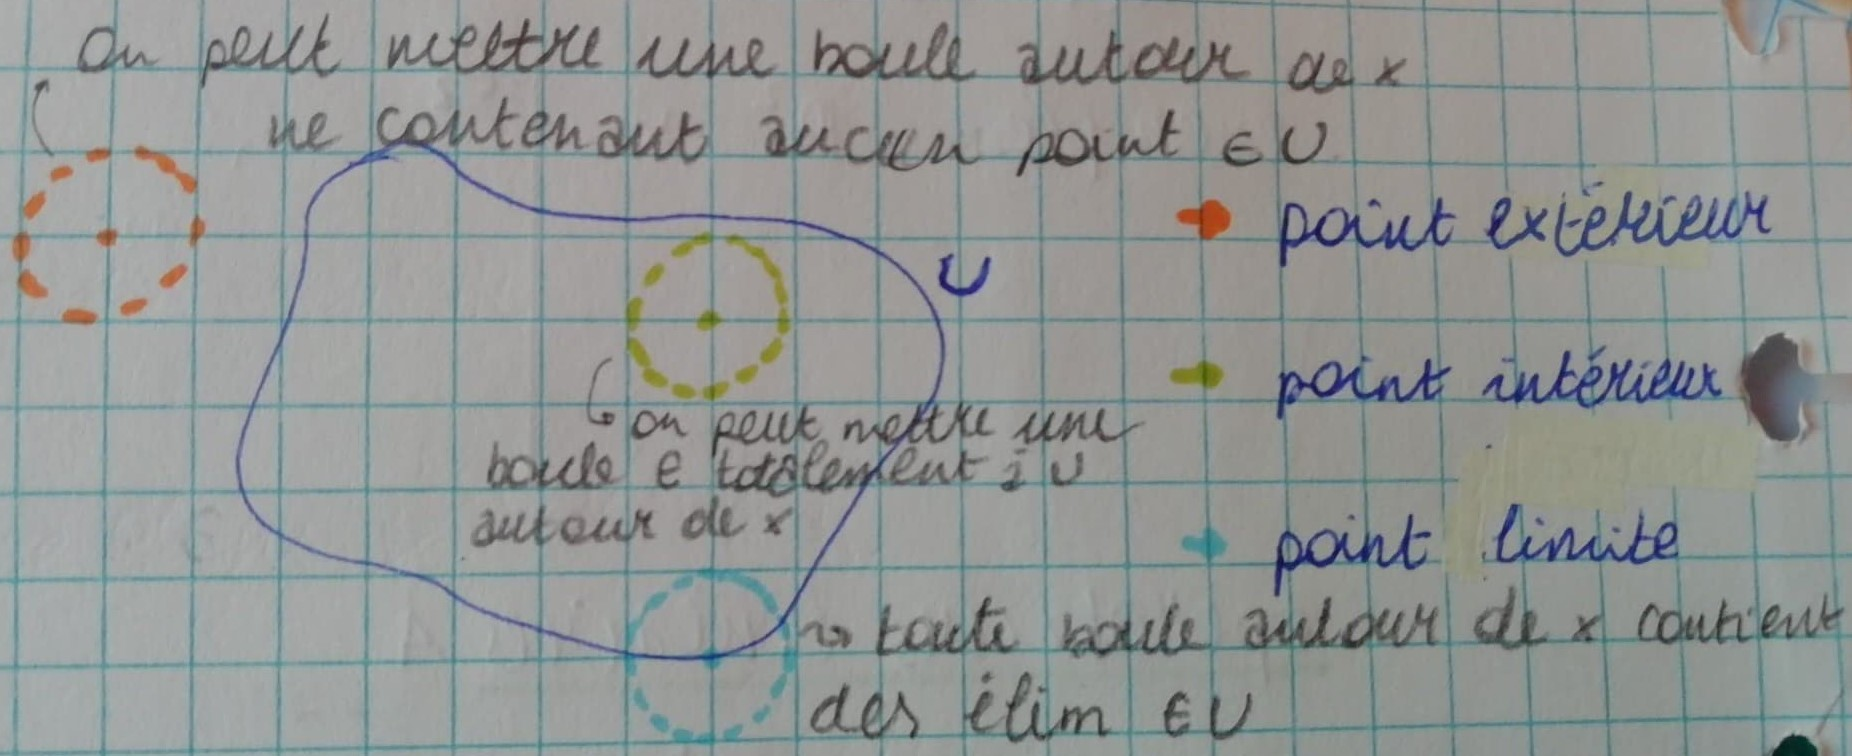
\includegraphics[scale = 0.3]{synthese_BO.jpg}
\end{figure}

\begin{definition}
    Un point $x\in U\subseteq X$ est un \textbf{point intérieur} à $U$ s'il existe $r>0$ tel que $B_r(x) \subseteq U$. De manière équivalente, $x$ est un point intérieur de $U$ si $U$ contient (entièrement !) une certaine balle en $x$.
\end{definition}

\begin{definition}
    Si $x$ est un point intérieur de $U$, alors $U$ est aussi appelé \textbf{voisinage} de $x$ (voisinage de $x$ = boule ouverte centrée en $x$).
\end{definition}

\begin{definition}
    Un point $x$ est appelé \textbf{point limite} de $U$ si $B_r(x)\cap \left(U\setminus \left\{x\right\}\right)\neq\emptyset$ pour toute balle autour de $x$. Notez qu'un point limite n'est pas spécialement un élément de $U$, mais $U$ doit contenir un point arbitrairement proche de $x$.
\end{definition}

\begin{remark}
    Un point intérieur est un point limite mais un point limite n'est pas toujours un point intérieur
\end{remark}

\begin{example}
    Le point $a$ est il point limite de l'ensemble $\{a,b\}$ ? Non car cet espace est un espace discret. Il existe donc une boule ne contenant aucun autre élément que $a$.
\end{example}

\begin{definition}
    Un point $x$ est un \textbf{point isolé} de $U$ s'il existe un voisinage de $x$ ne contenant aucun autre élément de $U$. Un espace contenant que des points isolés est un \textbf{espace discret}.
\end{definition}

\begin{definition}
    Si tout voisinage de $x$ contient au moins un élément de $U$ et un élément hors de $U$, alors $x$ est appelé \textbf{point frontière}. En mathématique, on écrit que $U\subseteq X$ si pour tout $r>0$
    \begin{equation*}
        \left\{\begin{array}{rcl}
            B_r(x)\cap U &\neq& \emptyset  \\
            B_r(x)\cap (X\setminus U) &\neq& \emptyset
        \end{array}\right.
    \end{equation*}
    L'ensemble de tous les points frontière de $U$ est appelé la frontière de $U$ \footnote{Étonnant, n'est-ce pas ?} et dénoté par $\partial U$.
\end{definition}

Un point frontière est-il toujours point limite ? Non. Prenons un point isolé $x$. Ce point est par définition un point frontière mais pas un point limite.

Un point frontière peut-il être point intérieur d'un même ensemble ? Non, car il est possible de trouver une boule (assez petite) en un point intérieur $x\in U\subseteq X$ qui ne contiennent aucun élément de $X \textbackslash U$. Ce point ne peut être point frontière, donc. De même, il est impossible de trouver une boule en un point frontière $y$ qui ne contienne aucun élémenent de $X$.

\begin{definition}
    Un ensemble dont tous les points sont des points intérieurs est appelé \textbf{ensemble ouvert} ; $U \subseteq X$ est \textbf{ouvert} si $\forall x \in U : \exists \ r > 0 : B_r(x) \subseteq U$
    \newpage
    La famille de tous les ensembles ouverts $\mathcal{O} \in$ à l'espace métrique $X$ satisfait les propriétés suivantes :
    \begin{enumerate}[label=(\roman*)]
        \item $\emptyset,X\in \mathcal{O}$ ;
        \item $O_1,O_2\in \mathcal{O}$ implique $O_1\cap O_2 \in \mathcal{O}$ ;
        \item $\left\{ O_\alpha \right\} \subseteq \mathcal{O}$ implique $\bigcup_\alpha O_\alpha \in \mathcal{O}$.
    \end{enumerate}
\end{definition}

\danger \textbf{Attention} :
    \begin{enumerate}[label=(\roman*)]
        \item Une intersection infinie d'ouvert n'est pas toujours un ouvert : $\bigcap \limits^\infty_{n=1}]\frac{-1}{n},1[ = [0,1[$
        \item Une intersection finie d'ouvert est toujours un ouvert
        \item Une union finie d'ouvert est toujours un ouvert
    \end{enumerate}
\vspace{0.3cm}

Un ensemble $X$ auquel est associé une famille $\mathcal{O}$ de sous-ensembles de $X$ qui satisfait les trois propriétés est appelé \textbf{espace topologique} : $(X, \mathcal{O})$ est un espace topologique de l'ensemble $X$ si la topologie $\mathcal{O} \subseteq \mathcal{P}(X)$ sur $X$ satisfait les 3 propriétés.\\

\begin{definition}
    Soit $(X,\mathcal{O})$ un espace topologique. Un ensemble $Y \subseteq X$ est un \textbf{sous-espace topologique} de $X$ s'il est muni de la \textbf{topologie induite}. C'est à dire, qu'un sous-ensemble $Z \subseteq Y$ est ouvert ssi il existe un ouvert $O \subseteq X$ tel que $Z = O \cap Y$.
\end{definition}

\begin{example}
    Soit $\mathbb{R}$ l'ensemble des réels muni de sa topologie naturelle. Soit $Y := [-1,1]$ le sous-espace topologique de $\mathbb{R}$ muni de la topologie induite. Si $Z = ]0,1]$, il suffit par exemple de prendre $O = ]0,a[$ avec n'importe quel réel $a > 1$.
    
    On remarque donc que $Z$ n'est pas un ouvert pour la topologie de $\mathbb{R}$ mais il l'est dans $Y$ pour la topologie induite.
\end{example}

\begin{remark}
    Le fait qu'un ensemble $Z$ soit ouvert ou fermé dans un ensemble $X$ ne dépend pas uniquement de l'ensemble $Z$ lui-même, ça dépend aussi de $X$!
\end{remark}

Les notions de point intérieur, de point limite et de voisinage se répercutent sur les espaces topologiques si nous remplaçons la boule ouverte autour de $x$ par un jeu ouvert contenant $x$. Il existe différents choix quant à la topologie, les plus évidents étant la \textbf{topologie triviale} $\mathcal{O} = \left\{ \emptyset,X \right\}$ et la \textbf{topologie discrète} $\mathcal{O} = \mathcal{P}(X)$.\\

\begin{definition}
    Un espace topologique $(X,\mathcal{O})$ est de \textbf{Hausdorff} si pour tout $x,y \in X$ ($x\neq y$), il existe $O_1,O_2$ tels que $x\in O_1\in \mathcal{O}$ et $y\in O_2\in \mathcal{O}$ avec $O_1\cap O_2=\emptyset$. Autrement dit, pour deux points distincts, il existe deux voisinages disjoints.
\end{definition}

%Dans un tel espace, si une suite a une limite, alors cette limite est unique.

\begin{theo}
    Si $U\subseteq X$ est fermé, alors $X\setminus U$ est ouvert.
\end{theo}

\begin{definition}
    La boule fermée de rayon $r$ centrée en $x$ est donnée par
    \begin{equation*}
        \overline{B_r}(x) := \left\{ y\in X| d(x,y) \leq r \right\}
    \end{equation*}
    Remarquez que $\overline{B_r}(x)$ n'est pas une adhérence !
\end{definition}

\begin{definition}
    Soit $U\subseteq X$ un ensemble. Le plus petit ensemble fermé contenant l'ensemble $U$, appelé \textbf{adhérence} ou \textbf{fermeture} de $U$ et est noté $\overline{U}$. Le plus grand ensemble ouvert contenu dans $U$ est appelé \textbf{intérieur} de $U$ et est noté $U \degree$
    
    Propriétés (démos TP3) :
    \begin{enumerate}[label=(\roman*)]
        \item $\overline \emptyset = \emptyset$,
        \item $U \subseteq \overline U$,
        \item $\overline{\overline U} = \overline U$,
        \item $\overline{U\cup V} = \overline U \cup \overline V$.
        \item $X \setminus \overline{U} = (X \setminus U)\degree$ et $X \setminus U\degree = \overline{X \setminus U}$
        \item $\partial U = \overline{U} \setminus U\degree$
    \end{enumerate}
\end{definition}

\begin{theo}
    \begin{equation*}
        \overline{B_r(x)} \subseteq \overline{B_r}(x).
    \end{equation*}
\end{theo}

\begin{example}
    Soit l'espace métrique $X := \{0,1\}$ muni de la distance $d(x,y) := |x-y|$. On a donc $\overline{B_1^X}(0) = \{0,1\}$ et $B_1^X(0) = \{0\}$. Donc, $\overline{B_1^X(0)} = \overline{\{0\}} = \{0\} \subseteq \{0,1\}$
\end{example}

%\begin{proof}
    %Cela équivaut à prouver que $X\setminus \overline{B_r}(x)\subseteq X\setminus \overline{B_r(x)}$. Prenons par exemple les points $x,y\in\mathbb{R}^2$ sur la Fig.\ref{fig:preuve1} tels que $d(x,y) = R$. Soit $B_r(x)$ la boule ouvert en $x$ de rayon $r<R$.
    %\begin{figure}
        %\centering
        %\tikzsetnextfilename{preuve1}
        %\begin{tikzpicture}
            %\draw[->] (-.5,0) -- (4,0) node[below] {\small{$e_1$}};
            %\draw[->] (0,-.5) -- (0,4) node[left] {\small{$e_2$}};

            %\draw plot[mark=*, mark size=.3mm] (1.6,1.3) node[above left] {\small{$x$}} circle(1) -- (2.3071,2.0071) node[above right] {\small{$r$}};
            %\draw (1.6,1.3) -- (3,1.7) node[above left] {\small{$R$}} -- plot[mark=*, mark size=.3mm] (3.6,1.9) node[above right] {\small{$y$}};
        %\end{tikzpicture}
        %\caption{}
        %\label{fig:preuve1}
    %\end{figure}
%\end{proof}

%\begin{theo}
    %Une famille d'ensembles ouverts $\mathcal{B}\subseteq\mathcal{O}$ est une \textbf{base} pour la topologie si et seulement si tous les ensembles ouverts peuvent être écrits comme une union des éléments de $\mathcal{B}$.
%\end{theo}

\subsection{Convergence}

\begin{definition}
    Une \textbf{sous-suite} (ou une \textbf{suite extraite}) d'une suite $(x_n)_{n\in\mathbb{N}}$ est une suite $(x_{n_k})_{k\in\mathbb{N}}$ où $(n_k)_{k\in\mathbb{N}}\subset \mathbb{N}$ est strictement croissante.
\end{definition}

\begin{definition}
    Dans un espace métrique $(X,d)$, la suite $(x_n)_{n\in\mathbb{N}}\subset X$ est \textbf{bornée} si et seulement si $\sup_{n\in\mathbb{N}}d(x_n,x_0)<\infty$. Autrement dit, $(x_n)_{n\in\mathbb{N}}\subset X$ est bornée si $\exists y \in X, r > 0 : \forall n \in \mathbb{N} : x_n \in B_r(y)$. 
\end{definition}

\begin{definition}
    Dans un espace métrique $(X,d)$, une suite $(x_n)_{n=1}^\infty$ \textbf{converge} vers un point $x\in X$ si $\lim \limits_{n\rightarrow\infty}d(x,x_n) = 0$. De manière équivalente, on dit qu'une suite $x_n$ converge si et seulement s'il existe $x\in X$ tel que pour tout réel $\epsilon>0$, il existe $N\in\mathbb{N}$ tel que $d(x_n,x) \leq \epsilon$ (ou $x_n \in B_\epsilon(x)$) pour tout entier $n\geq N$. Il semble évident que cette limite est unique, si elle existe.
\end{definition}

\begin{definition}
    Soit une suite $(u_n)_{n \in \mathbb{N}}$ de fonctions d’un ensemble $X$ dans un espace métrique $(Y, d)$.
    
    La suite \textbf{converge ponctuellement} vers $u(x)$ si
    \begin{equation*}
        \exists u : X \rightarrow Y \ \text{telle que} \lim \limits_{n\to\infty} d(u_n(x), u(x)) = 0 \quad \forall x \in X
    \end{equation*}
    
    
    La suite \textbf{converge uniformément} vers $u(x)$ si
    \begin{equation*}
        \exists u : X \rightarrow Y \ \text{telle que} \lim \limits_{n\to\infty} \sup \limits_{x \in X} \{d(u_n(x), u(x))\} = 0
    \end{equation*}
    
    La convergence uniforme implique la convergence ponctuelle mais pas le contraire
\end{definition}

\noindent
\fbox{\parbox{\textwidth}{%\raggedleft
    \begin{exo}
        Soit $(x_n)_{n\in\mathbb{N}}$ une suite de nombres réels décroissante et bornée. Prouver que $(x_n)_{n\in\mathbb{N}}$ converge et
        \begin{equation*}
            \lim_{n\to\infty}x_n = \inf\{x_n:n\in\mathbb{N}\}
        \end{equation*}
    \end{exo}
    \begin{sol}
        Soit $N = \inf\{x_n:n\in\mathbb{N}\}$. Comme la suite est bornée, nous déduisons que $N\in\mathbb{R}$ existe. La suite étant décroissante, nous avons $d(x_n,N) \geq d(x_m,N)$, $\forall m > n$. En choisissant $\epsilon = d(x_n,N) > 0$, on peut affirmer que la suite converge uniformément vers $N$.
    \end{sol}
}}\\

\begin{theo}[Bolzano-Weierstrass]
    Tout suite bornée admet une sous-suite convergente. (démo au TP2) \danger Pas valable en dimension infinie !
\end{theo}

Il est à noter qu'une suite convergente est bornée. Un ensemble $U\subset X$ est \textbf{borné} s'il est contenu dans une balle, c'est-à-dire $U\subset B_r(x)$ pour certains $x\in X$ et $r>0$. \\

%Une métrique induit naturellement une topologie et une topologie induit naturellement une notion de convergence. Cependant, une notion de convergence peut ne pas provenir d'une topologie (ou différentes topologies peuvent donner lieu à la même notion de convergence) et une topologie peut ne pas provenir d'une métrique.

\begin{definition}
    Une suite $(x_n)_{n=1}^\infty\in X^\mathbb{N}$ est appelée \textbf{suite de Cauchy} si pour chaque $\epsilon>0$, il existe $N\in\mathbb{N}$ tel que
    \begin{equation*}
        d(x_n,x_m)\leq\epsilon,\qquad n,m\geq N.
    \end{equation*}
\end{definition}

\begin{theo}
    Toute suite convergente est de Cauchy.
\end{theo}

\noindent
\fbox{\parbox{\textwidth}{%\raggedleft
    \begin{exo}
        Démontrer que dans un espace métrique, toute suite de Cauchy est bornée.
    \end{exo}
    \begin{sol}
        Soit la suite $(u_n)_{n=1}^\infty$ qui converge uniformément vers $u$. On a alors, par inégalité triangulaire, que
        \begin{equation*}
            0\leq d(u_j,u_k)\leq d(u_j,u) + d(u,u_k)
        \end{equation*}
        et $\lim \limits_{j,k\to\infty} d(u_j,u_k) = 0$. Si cette suite est de Cauchy, pour un certain $\epsilon>0$, il existe alors $m\in\mathbb{N}$ tel que $j,k\geq m$ et $d(u_j,u_k)\leq\epsilon$. On obtient alors pour tout $n$
        \begin{equation*}
            d(u_0,u_n) \leq \max\{ d(u_0,u_1), \cdots , d(u_0,u_{m-1}), d(u_0,u_m)+\epsilon \}.
        \end{equation*}
    \end{sol}
}}\\

\begin{definition}
    Une suite $(x_n)_{n\in\mathbb{N}}$ de nombres réels est \textbf{sommable} si la suite $\Big(\sum \limits_{k=0}^n x_k\Big)_{n\in\mathbb{N}}$ converge.
\end{definition}

\begin{definition}
    La limite $\lim \limits_{n\to\infty}\sum \limits_{k=0}^n x_k = \sum \limits_{k=0}^\infty x_k$ est appelée \textbf{somme} de la série de terme $x_n$.
\end{definition}    

\begin{definition}
    $\sum \limits_{k=0}^\infty x_k$ converge si la suite $(x_n)_{n\in\mathbb{N}}$ est sommable. Dans le cas contraire, la série est dite \textbf{divergente}.\\
    
    Les définitions de convergence ponctuelle et uniforme restent valables pour les séries en regardant la convergence de la suite $\Big(\sum \limits_{k=0}^n x_k\Big)_{n\in\mathbb{N}}$\\
    
    La série $\sum \limits_{k=0}^n x_k$ où $(x_k)_{k\in\mathbb{N}}$ est une suite de Y dans un espace normé (cf plus loin) \textbf{converge absolument ponctuellement} si
    \begin{equation*}
         \sum \limits_{k=0}^n ||x_k(y)|| < \infty \quad \forall y \in Y
    \end{equation*}
    
    La série $\sum \limits_{k=0}^n x_k$ où $(x_k)_{k\in\mathbb{N}}$ est une suite de Y dans un espace normé (cf plus loin) \textbf{converge normalement} si
    \begin{equation*}
         \sum \limits_{k=0}^n \sup \limits_{y \in Y}||x_k(y)|| < \infty
    \end{equation*}
    
    La convergence normale implique la convergence absolue ponctuelle.
\end{definition}

\subsection{Caractérisation des fermés}

$U\subseteq X$ est fermé si pour toute suite $(x_n)_{n=1}^\infty\subseteq U$ et $x_n\rightarrow x$, alors $x\in U$.

\begin{definition}
    Un espace métrique $X$ est \textbf{complet} si toute suite de Cauchy converge avec limite dans $X$.
\end{definition}

\noindent
\fbox{\parbox{\textwidth}{%\raggedleft
    \begin{exo}
        Prouver que $\mathbb{Q}$ muni de la distance $d(x,y)=|x-y|$ n'est pas complet.
    \end{exo}
    \begin{sol}
        Considérons la suite $(x_n)_{n\in\mathbb{N}}$ définie par
        \begin{equation*}
            x_0=2,\quad x_{n+1} = \frac{1}{2}\left(x_n + \frac{2}{x_n}\right)
        \end{equation*}
        Prouvons d'abord que cette suite est de Cauchy. Pour ce faire, étudions la suite afin de voir si elle croissante ou décroissante :
        \begin{equation*}
            x_{n+1} - x_n = \frac{2-x_n^2}{x_n} \overset{?}{\gtrless} 0
        \end{equation*}
        On en déduit que la fonction est décroissante positive et qu'elle converge vers $\sqrt{2}$, c'est-à-dire dans $\mathbb{R}$. On en conclut que $\mathbb{R}$ est complet, mais pas $\mathbb{Q}$.
    \end{sol}
}}\\

\begin{lemme}
    Soit $X$ un espace métrique complet et $U\subseteq X$. On a :
    \begin{equation*}
        U\ \mathrm{complet} \quad\Longleftrightarrow\quad U\ \mathrm{ferm\acute{e}}
    \end{equation*}
\end{lemme}

\begin{definition}
    L'espace métrique $U\subseteq X$ est \textbf{dense} si et seulement si $\overline{U}=X$. Autrement dit, $U$ est dense dans $X$ ssi $\forall x \in X, \forall r>0 : B_r(x) \cap U \neq \emptyset$
\end{definition}

\begin{lemme}
    L'espace métrique $X$ est \textbf{séparable} si et seulement s'il contient un ensemble dense dénombrable.
\end{lemme}

\begin{example}
    $\mathbb{Q}$ est dense dans $\mathbb{R}$ (imaginons une infinité de frontières entre chaque éléments de $\mathbb{Q}$). L'ensemble $\mathbb{Q}$ est également dénombrable. On a donc que $\mathbb{R}$ est séparable.
\end{example}

\subsection{Fonctions}

\begin{definition}
    une fonction $f$ est la relation d'un ensemble $X$ vers un ensemble $Y$ pour laquelle chaque élément $x\in X$ est en relation avec un unique élément du second, appelé image de $x$ et noté $f(x)$. C'est-à-dire
    \begin{equation*}
        f:X\rightarrow Y,\ x\mapsto f(x).
    \end{equation*}
    On écrit généralement $f(U) = \left\{ f(x)|x\in U \right\}$ pour $U\subseteq X$ et $f^{-1}(V) = \left\{ x|f(x)\in V \right\}$ pour $V\subseteq Y$.
\end{definition}

\begin{figure}[H]
    \centering
    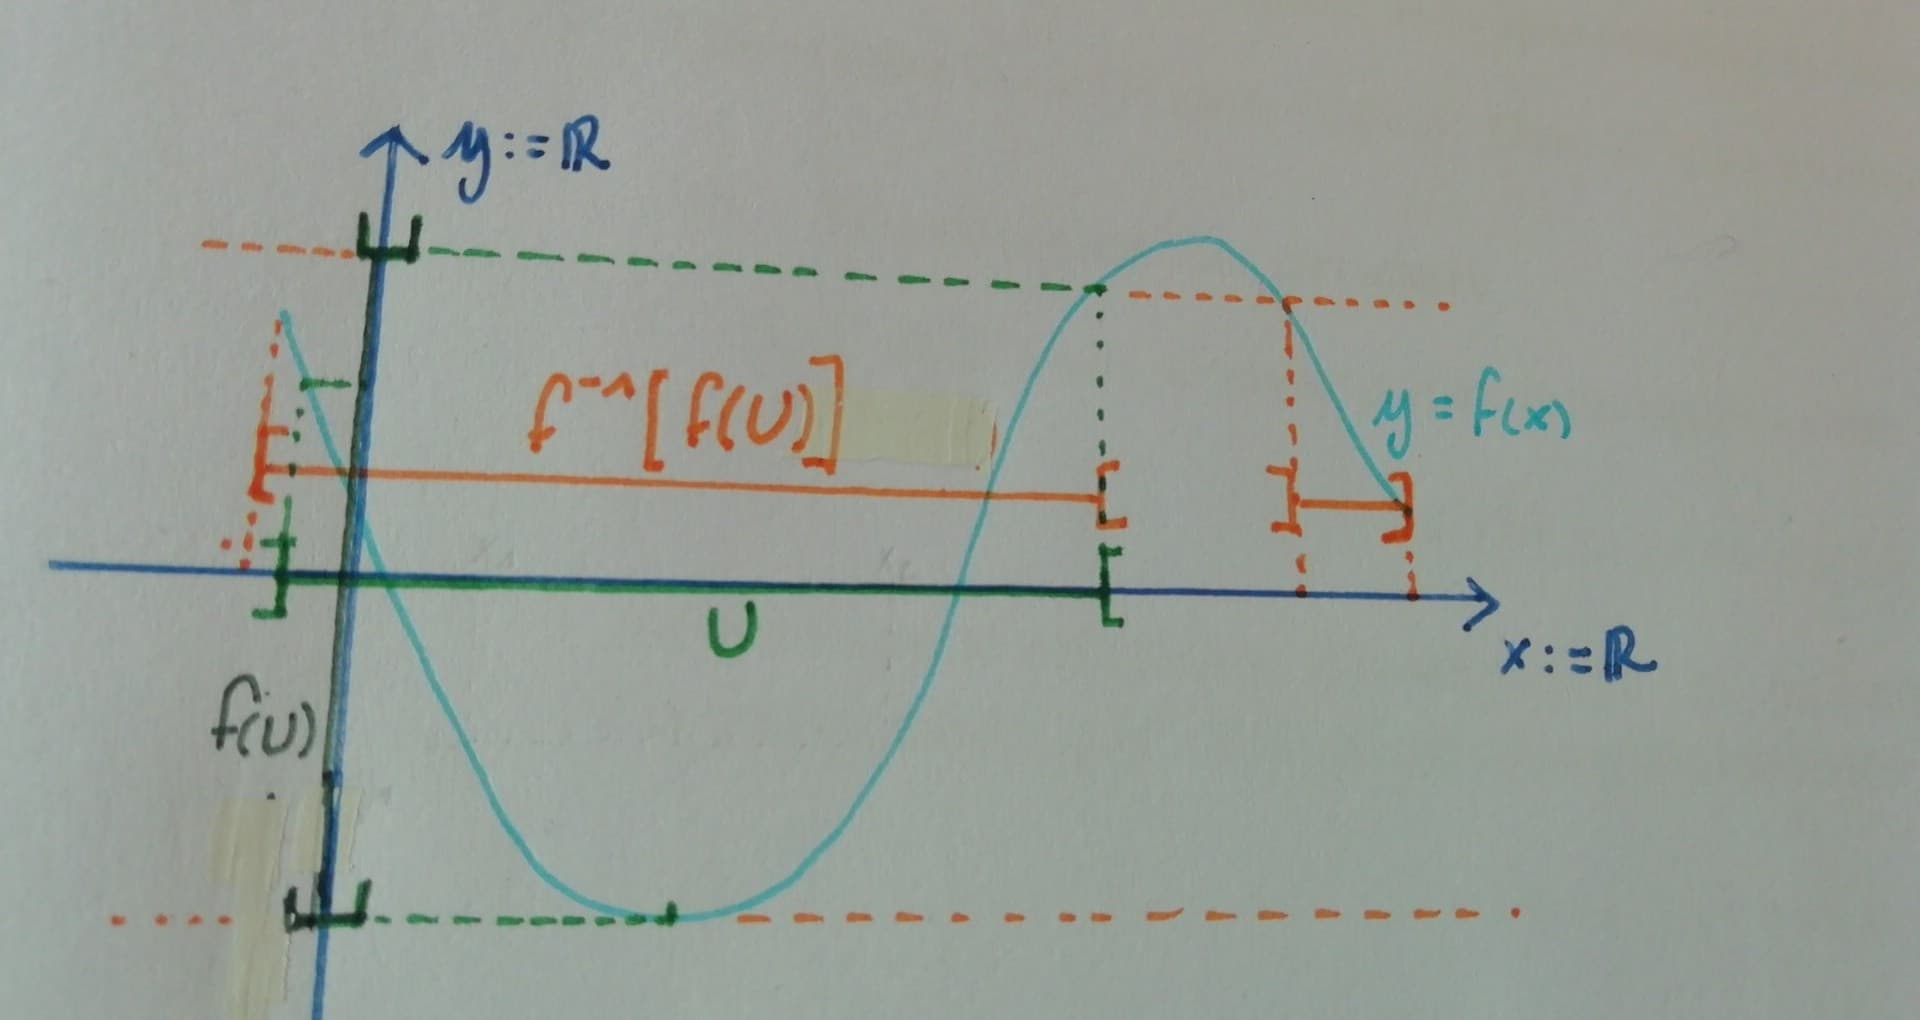
\includegraphics[scale = 0.1]{synthese_fct.jpg}
\end{figure}

\begin{definition}
    On dit qu'une fonction $f$ est
    \begin{itemize}
        \item \textbf{injective} si pour chaque $y \in Y$, il y a au plus un $x \in X$ tel que $f(x) = y$ ($f^{-1}(y)$ contient au plus un point);
        \item \textbf{surjective} si $f(X)=Y$;
        \item \textbf{bijective} si elle est à la fois injective et surjective.
    \end{itemize}
\end{definition}

\begin{definition}

    Une fonction $f$ entre deux espaces métriques $X$ et $Y$ est dite continue en un point $x\in X$ si pour tout $\epsilon>0$, on peut trouver un $\delta>0$ tel que $d_Y(f(x),f(y)) \leq \epsilon \quad\mathrm{si}\quad d_X(x,y)<\delta$ ou de manière équivalente : $f(B_\delta(x)) \subseteq B_\epsilon(f(x))$.\\
    \begin{figure}[H]
        \centering
        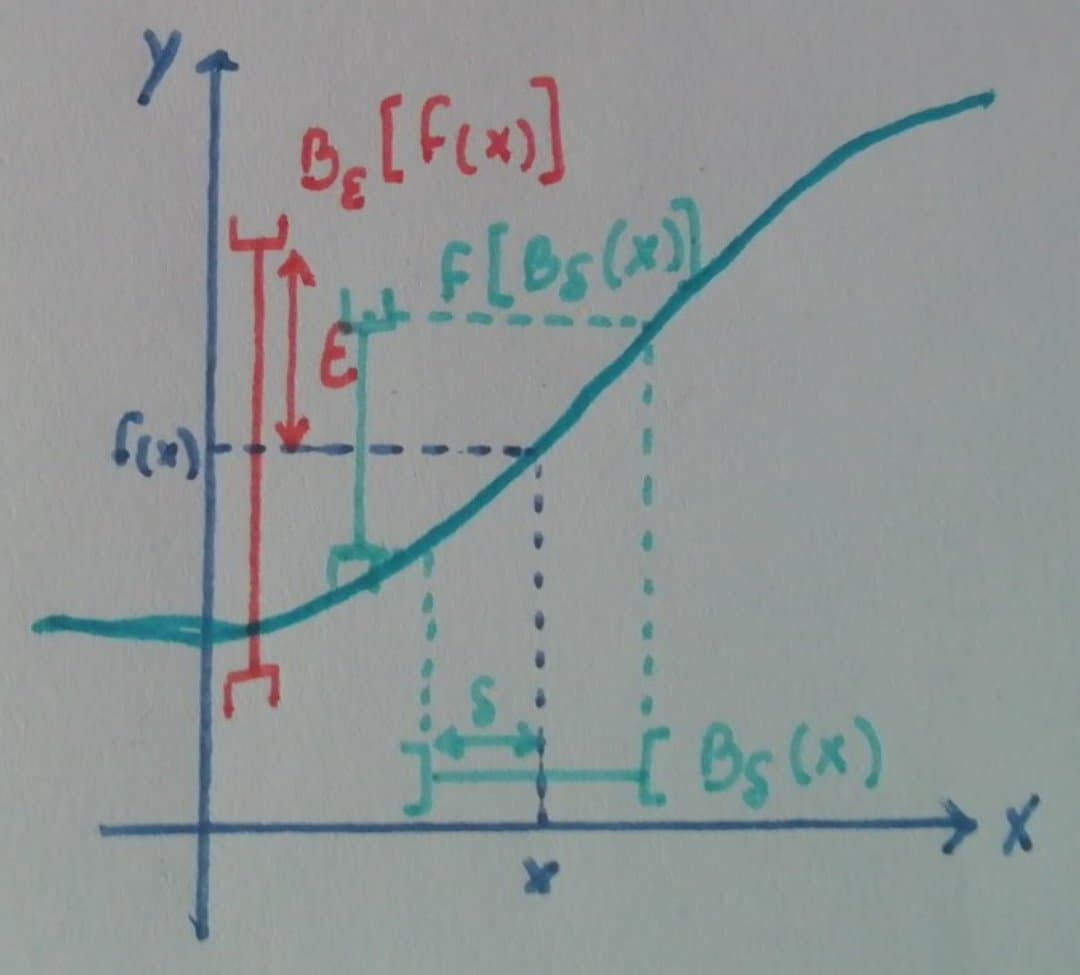
\includegraphics[width=0.3\textwidth]{synthese_continuite.jpg}
    \end{figure}
    Si $f$ est continue en chaque point, on dit qu'elle est \textbf{continue}.
\end{definition}

\begin{definition}
    Une fonction $f:X \rightarrow Y$ avec $X$ et $Y$ deux espaces métriques muni des distance $d_X$ et $d_Y$ respectivement est \textbf{uniformément continue} si $\forall \epsilon>0, \exists \delta>0$ tels que $\forall x,y \in X : d_X(x,y) \leq \delta \implies d_Y(f(x),f(y))\leq \epsilon$.
\end{definition}

\begin{theo}
    Soient $X,Y$ deux espaces métriques. Les déclarations suivantes sont équivalentes :
    \begin{enumerate}[label=(\roman*)]
        \item $f$ est continue en $x$ ;
        \item $f(x_n)\rightarrow f(x)$ pour n'importe quel $x_n \rightarrow x$ ;
        \item Pour tout voisinage $V$ de $f(x)$, la pré-image $f^{-1}(V)$ est un voisinage de $x$.
    \end{enumerate}
\end{theo}

\begin{proof}

    $1.\Rightarrow2.$ Soit un réel $\epsilon>0$. Par continuité de $f$, il existe $\delta>0$ tel que $f(B_\delta(x))\subseteq B_\epsilon(f(x))$. Par convergence de $(x_n)$ vers $x$, il existe $N$ tel que $\forall n\geq N$ :
    \begin{equation*}
        x_n\in B_\delta(x) \Rightarrow f(x_n)\in f(B_\delta(x)) \subseteq B_\epsilon(f(x))
    \end{equation*}
    
    $2.\Rightarrow3.$ Par contradiction : Soit $V$ un voisinage de f(x) tel que $f^{-1}(V)$ n'est pas un voisinage de $x$ ($\forall \delta > 0: B_\delta(x) \not\subseteq f^{-1}(V)$). Dans ce cas, on peut choisir une suite $x_n \in B_{\frac{1}{n}}(x)$ qui converge vers $x$ telle que $f(x_n) \notin V$ et donc $f(x_n) \nrightarrow f(x)$.\\
    \begin{figure}[H]
        \centering
        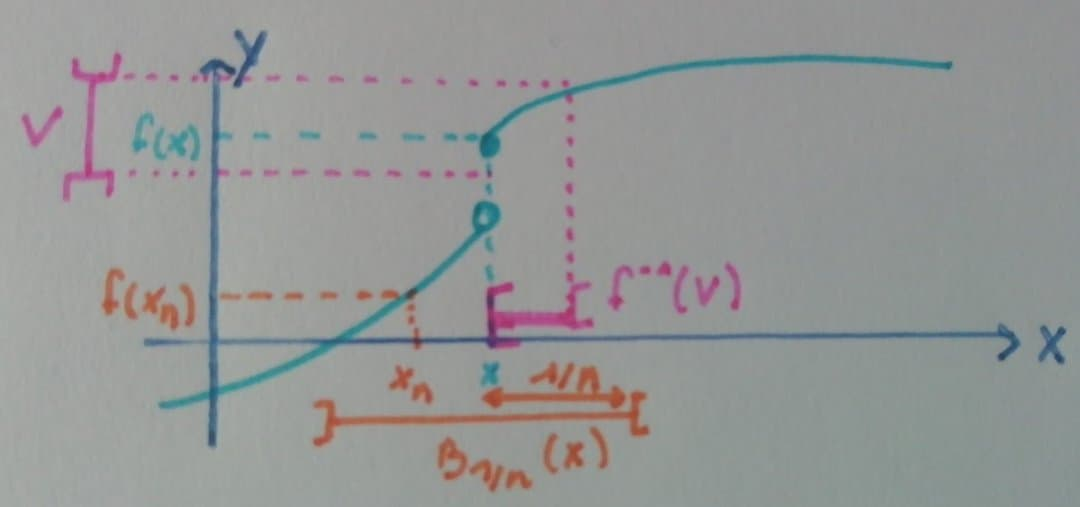
\includegraphics[scale = 0.2]{synthese_continuite_theo.jpg}
    \end{figure}
    
    $3.\Rightarrow1.$ Soit un voisinage V autour de $f(x)$ : $V = B_\epsilon(f(x))$, $\epsilon > 0$. Dès lors, $f^{-1}(V) = f^{-1}(B_\epsilon(f(x)))$ est un voisinage de x donc $\exists\delta : B_\delta(x)\subseteq f^{-1}(B_\epsilon(f(x)))$, c'est-à-dire que $f$ est continue en $x$.
\end{proof}

\begin{remark}
	$f:X\rightarrow Y$ est continue si et seulement si $\forall \mathcal{O}$ ouvert de $Y:f^{-1}(\mathcal{O})$ est un ouvert de $X$.
\end{remark}

%\begin{definition}
	%La fonction $f$ est un \textbf{homéorphisme} si et seulement si elle est bijective et que $f$ et $f^{-1}$ sont continues.
%\end{definition}

\begin{definition}
    Le \textbf{support} de la fonction f est défini comme
	\begin{equation*}
		\text{supp}(f):=\overline{\{x\in X|f(x)\neq0\}}
	\end{equation*}
\end{definition}

\subsection{Compacité}

\begin{definition}
	Un \textbf{recouvrement} de $Y\subseteq X$ est une famille d'ensembles $\{U_\alpha\}_{\alpha\in A}$ telle que $Y\subseteq \bigcup_{\alpha\in A}U_\alpha$. Le recouvrement est \textbf{ouvert} si tous les $U_\alpha$ sont ouverts. Un \textbf{sous-recouvrement} est une sous-famille de $\{U_\alpha\}$ qui reste un recouvrement de $Y$. 
\end{definition}

\begin{figure}[H]
    \centering
    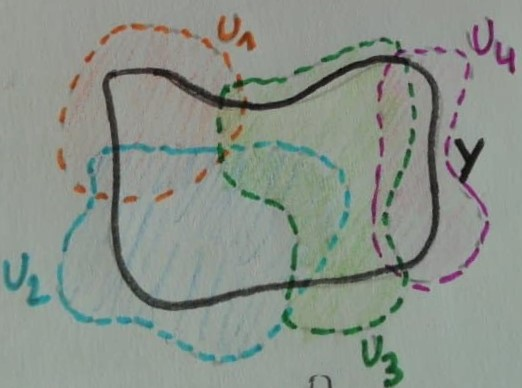
\includegraphics[scale = 0.4]{synthese_recouvrement.jpg}
\end{figure}

\begin{definition}
    Un ensemble $K\subseteq X$ est \textbf{compact} si \underline{tout} recouvrement \textit{ouvert} de $K$ a un sous-recouvrement fini. (Un espace est non compact si il est trop grand ex. $\mathbb{R}$)
\end{definition}

\begin{theo}
    Soit un espace topologique $X$.
    \begin{enumerate}[label=(\roman*)]
        \item L'image continue d'un ensemble compact est compacte.
        \item Tout sous-ensemble fermé d'un ensemble compact est compact.
        \item Si $X$ est de Hausdorff, tout ensemble compact est fermé.
    \end{enumerate}
\end{theo}

\begin{proof}
    \begin{enumerate}
        \item Observons que si $\{O_\alpha\}$ est un recouvrement fermé de $f(Y)$, alors $\{f^{-1}(O_\alpha)\}$ en est un pour $Y$.
        \begin{figure}[H]
            \centering
            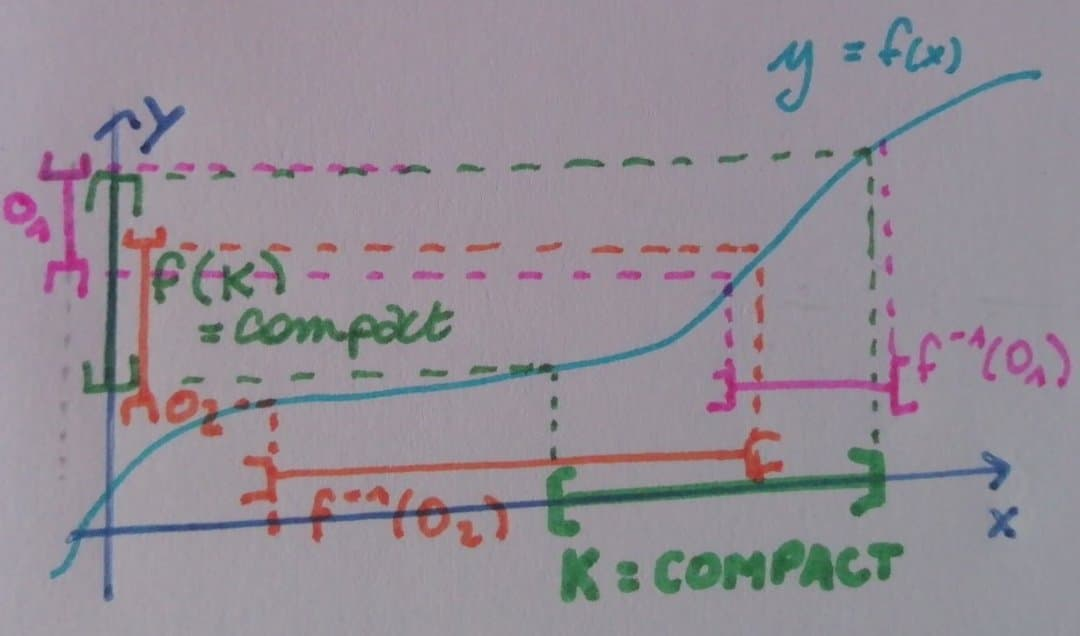
\includegraphics[scale = 0.2]{synthese_compact.jpg}
        \end{figure}
        \item Soit $\{O_\alpha\}$ un recouvrement ouvert d'un sous-ensemble fermé $Y$. Alors, il existe des ensembles ouverts $\tilde{O}_\alpha$ avec $O_\alpha = \tilde{O}_\alpha\cap Y$ et $\{\tilde{O}_\alpha\}\cup\{X\setminus Y\}$ (un recouvrement ouvert de $X$) qui sont un sous-recouvrement fini. Ce sous-recouvrement implique un sous-recouvrement fini de $Y$.
        \item Soit $Y\subseteq X$ un compact. On montre que $X\setminus Y$ est ouvert. Fixons $x\in X\setminus Y$. Comme l'ensemble $X$ est de Hausdorff, pour chaque $y\in Y$ (donc $\in X$), il y a un voisinage disjoint $V(y)$ de $y$ et $U_y(x)$ de $x$. Comme $Y$ est compact, il existe $y_1,\cdots,y_n$ tels que $V(y_j)$ recouvre $Y$. Mais alors $\bigcap_{j=1}^n U_{y_j}(x)$ est un voisinage de $x$ qui n'a aucune intersection avec $Y$.
    \end{enumerate}
\end{proof}

\begin{definition}
    L'ensemble $K\subseteq X$ est \textbf{séquentiellement compact} si toute suite dans $K$ a au moins une sous-suite convergente dont la limite est dans $K$.
\end{definition}

\begin{definition}
    L'ensemble $K\subseteq X$ est \textbf{séquentiellement fermé} si toute suite dans $K$ converge dans $K$.
\end{definition}

\begin{theo}
    Tout ensemble $K\subseteq X$ est compact (fermé) si et seulement s'il est séquentiellement compact (fermé).
\end{theo}

\begin{theo}
    Un espace métrique compact est complet et séparable.
\end{theo}

\begin{theo}
    Un espace métrique compact est fermé et borné (démo TP8).
\end{theo}

\begin{theo}[Heine-Borel]
    Dans $\mathbb{R}^n$, un ensemble est compact si et seulement s'il est fermé et borné.
\end{theo}

\subsection{Topologies du produit}

Si $X$ et $Y$ sont deux espaces métriques, alors $X\times Y$ associé à \[d((x_1,y_1),(x_2,y_2)) := d_X(x_1,x_2) + d_Y(y_1,y_2)\] est un espace métrique. Une suite $(x_n,y_n)_{n \in \mathbb{N}}$ converge vers $(x,y)$ si et seulement si $x_n\rightarrow x$ et $y_n\rightarrow y$. En particulier, par l'inégalité triangulaire inverse, on a \[|d(x_n,y_n) - d(x,y)| \leq d(x_n,x) + d(y_n,y)\] on voit que $d:X\times X \rightarrow \mathbb{R}$ est continue.
